\section{MPI One-Sided Communication}
\subsection{Required submission files}
\begin{enumerate}
  \item \hl{The updated \emph{gauss.c} file.}

  \item \hl{The new performance plots and description in the report.}

\end{enumerate}

\subsection{Questions}
\begin{enumerate}
  \item \hl{Which MPI-IO operations were applied to transform the code? Explain your choices.}
  There were several MPI-IO operations chosen to replace different parts of the code
  \begin{enumerate}
  \item 1) Reading in the matrix.
  
  We used an \verb!MPI_Read! function to read the first two ints at the beginning of the matrix to determine matrix dimensions. We then used an \verb!MPI_File_set_view! to separate the file into chunks and an \verb!MPI_File_read_all! for all processes to read in the required matrix data. We chose to use \verb!MPI_File_set_view! as the performance increase from a simple \verb!MPI_Read_at_all! was significant.
  
  We used \verb!MPI_File_set_view! and \verb!MPI_Read_all! to read in the rhs data as well.
  
  \item 2) Writing the resulting solution vector
  We used an \verb!MPI_Write! in the root process to store the output vector size. We then used \verb!MPI_File_set_view! and \verb!MPI_Write_all! so that each process could write to the correct segment in the file. We output doubles in binary.
  
  \end{enumerate}
  
  \item \hl{What is "Data Sieving" and "2-Phase IO"? How do they help improve IO
performance?}
	\begin{enumerate}
	\item Data Sieving
	
	Data sieving is performed by reading a large contiguous chunk of data into a memory buffer. Small chunks of non-contiguous data can then be read from or written to in the buffer. The entire buffer can then be written back to the filesystem if write operations have taken place.  
	
	The possible benefits are that, if a large number of small, non-contiguous data chunks are required, this will reduce the overhead of repeated communication of small segments of data. However, the downside is the large amount memory required as a larger chunk is loaded into memory than needed.
	
	\item 2-Phase IO
	
	This is also known as collective buffering. File accesses are performed by specific processes where data is aggregated. This works for both reading and writing. When reading, only certain processes will read large chunks of contiguous data---which is then communicated to the necessary processes. When writing, large chunks of data are aggregated in specific processes, which then write to file.
	
	Effectively, this ensures that file accesses are large and contiguous, significantly reducing IO time as opposed to performing many file accesses to small chunks of non-contiguous data. This does incur an additional communication cost/step but IO access is often far slower and the benefits of large contiguous file access outweights that of communication.
	\end{enumerate}

  \item \hl{Was the original implementation scalable in terms of IO performance?}
  The original implementation was not scalable in terms of IO performance. Only one process would read or write data. Thus, time would remain the same for IO regardless of the number of MPI processes.
  
  \item \hl{Was the original implementation scalable in terms of RAM storage?}
  The original implementation was not scalable in terms of RAM. When the program is run on a distributed memory system the entire matrix must fit inside the RAM associated with the processing unit executing the root process. This problem would not change regardless of the number of processing units (with their own memory) added.
  
  \item \hl{How much of the communication in the application was replaced or eliminated with MPI-IO? (Use
Vampir)}

  \item \hl{Were there any performance improvements due to the change to MPI-IO?}
  Yes, there was some performance improvements due to MPI-IO. We implemented the changes to MPI-IO on the baseline case to highlight the improvements.

\end{enumerate}
% % Figure example
% \begin{figure}[p] % h=here, t=top, b=bottom, p=(extra)page, !=force
%    \begin{center}
%      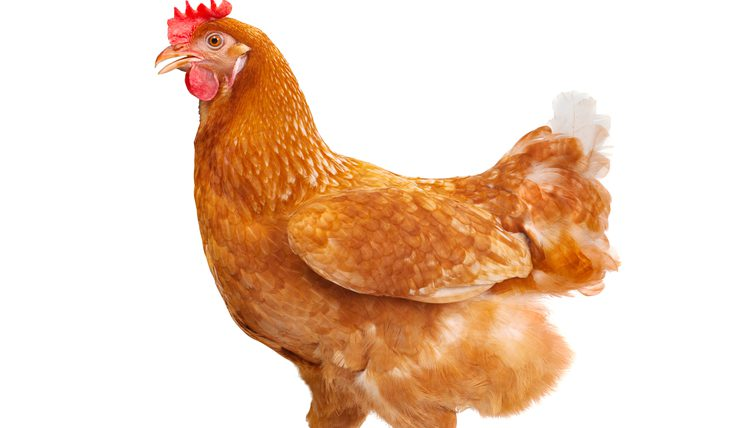
\includegraphics[width=.9\linewidth]{figure.png} % It searches in the Figures/ folder!
%      \caption{Caption text}
%      \label{fig:figureLabelName}
%    \end{center}
% \end{figure}
